%--- using \usetikzlibrary{automata}
%\newpage
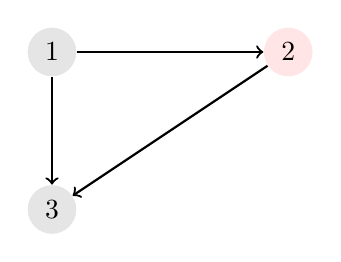
\begin{tikzpicture}
	\tikzstyle{vertex}=[circle,fill=black!10]
	\tikzstyle{selected vertex}=[vertex,fill=red!10]
	\tikzstyle{edge}=[->,thick]
	
	\node[vertex](v1) at (0,0){1};
	\node[selected vertex](v2) at (3,0){2};
	\node[vertex](v3) at (0,-2){3};	
	
	\draw[edge](v1)--(v2);
	\draw[edge](v1)--(v3);
	\draw[edge](v2)--(v3);	
\end{tikzpicture}
\caption{Example1}

\vspace{30pt}

\begin{tikzpicture}[->,node distance=3cm,auto]
	\node[initial,state](A){$q_1$};
	\node[state](B)[right of=A]{$q_2$};
	\node[state](C)[right of=B]{$q_3$};
	\node[state,accepting](D)[below of=B]{$q_4$};
	
	\path(A)edge[loop above]node{$1\rightarrow H,L$}(A)
			edge [bend left] node{$H \rightarrow 1,R$}(B)
		 (B)edge[loop above]node{b}(B)
		    edge [bend left] node{$H \rightarrow 1,L$}(A)
			edge node{$x_1$}(C)
    	 (C)edge[loop above]node{b}(C)
    	    edge node{$x_2$}(D)
	;	
\end{tikzpicture}
\caption{Example2}

\vspace{30pt}

\begin{tikzpicture}[->,node distance=3cm,auto]
	\node[initial,state](A){$A$};
	\node[state](B)[right of=A]{$B$};
	\node[state](C)[below of=A]{$C$};
	\node[state](D)[below of=B]{$D$};
	\node[state](E)[right of=D]{$E$};
	
	\path(A)edge[bend left](B)
	        edge(B)		 
		 (B)edge[bend left](A)
			edge(D)
    	 (C)edge(A)
    	    edge[loop below](C)
    	 (D)edge(C)
    	    edge(E)  
	;	
\end{tikzpicture}
\caption{This is node graph}